\section{Experimental Evaluation}
\label{sec:experimental-results}

This section presents a comprehensive experimental evaluation of memory-aware chunking across diverse workloads and deployment scenarios.
The evaluation addresses three fundamental questions that determine the practical viability of our approach:

\textbf{(Q1) Reliability:} Does memory-aware chunking eliminate \ac{OOM} failures across different data sizes and worker configurations?
This question addresses the primary motivation for our work, ensuring robust execution in memory-constrained environments.

\textbf{(Q2) Performance:} What is the execution time overhead compared to aggressive chunking strategies?
While memory safety is crucial, excessive performance degradation would limit practical adoption.

\textbf{(Q3) Robustness:} How sensitive is the method to prediction errors and safety factor selection?
Real-world deployments must handle variability in memory usage and system conditions.

\subsection{Setup}

\subsection{Experimental Setup}

Experiments were conducted on a dedicated \ac{HPC} node to ensure reproducible results without interference from other workloads.
The test system featured an Intel Xeon Silver 4310 processor (12 cores, 2.10 GHz) with 256~\ac{GB} DDR4 \ac{RAM}, running Ubuntu 20.04 LTS with Linux kernel 5.4.
We used Dask 2023.5.0 with NumPy 1.24.3 and Python 3.9.16.

The evaluation focused on the \ac{GST3D} operator, a memory-intensive kernel widely used in seismic attribute analysis.
\ac{GST3D} computes directional derivatives and their outer products, generating a 3×3 symmetric tensor at each voxel, a 6× memory expansion from the input.
We processed synthetic seismic volumes with dimensions ranging from $100^3$ (3.8 \ac{MB}) to $400^3$ (244 \ac{MB}), representing typical subvolumes in production workflows.

Each experiment varied the number of Dask workers from 1 to 8, with the available 32 \ac{GB} of \ac{RAM} evenly distributed among workers (32 \ac{GB} for 1 worker, 16 \ac{GB} each for 2 workers, 8 \ac{GB} each for 4 workers, and 4 \ac{GB} each for 8 workers).
This configuration mimics typical \ac{HPC} deployments where multiple workers share a single node's memory resources.
We compared three chunking strategies:

\textbf{(i) Auto (Dask default):} Targets 128 \ac{MB} chunks regardless of operator characteristics.

\textbf{(ii) Evenly-split:} Divides each dimension by the number of workers, creating regular partitions.

\textbf{(iii) Memory-aware:} Our proposed method using trained predictors with safety factor 0.8.

Each configuration was executed 5 times, with memory usage sampled at 100ms intervals using the process-level \ac{RSS} (Resident Set Size) metric.
Execution times exclude initial data loading to focus on computation performance.

\subsection{Reliability (Q1)}

Table~\ref{tab:oom-analysis} shows that memory-aware chunking prevented every \ac{OOM} failure recorded for the baselines (243 for Auto and 128 for Evenly-split across 768 trials).

\begin{table}[htb]
    \centering
    \caption{Out-of-memory incidents by chunking strategy}
    \label{tab:oom-analysis}
    \begin{tabular}{lccc}
        \toprule
        \textbf{Chunking Mode} & \textbf{\ac{OOM} Failures} & \textbf{Total Runs} & \textbf{\ac{OOM} Rate} \\
        \midrule
        Auto & 243 & 768 & 31.6\% \\
        Evenly-split & 128 & 768 & 16.7\% \\
        Memory-aware & 0 & 768 & 0.0\% \\
        \bottomrule
    \end{tabular}
\end{table}

\subsection{Performance and Memory Usage (Q2)}

When all methods succeeded, execution times differed by at most 65~\%.
Table~\ref{tab:overall-performance} lists median values.
For large volumes and four or more workers, only memory-aware completed, producing higher effective throughput overall (Figure~\ref{fig:performance-scaling}).

\begin{table}[htb]
    \centering
    \caption{Performance comparison for successful runs (median values)}
    \label{tab:overall-performance}
    \begin{tabular}{lccc}
        \toprule
        \textbf{Chunking Mode} & \textbf{Time (s)} & \textbf{Memory (\ac{GB})} & \textbf{Successful Runs} \\
        \midrule
        Auto & 15.7 & 2.62 & 525 \\
        Evenly-split & 15.7 & 2.63 & 640 \\
        Memory-aware & 28.1 & 1.24 & 768 \\
        \bottomrule
    \end{tabular}
\end{table}

The most striking difference lies in memory consumption.
Memory-aware chunking halved peak memory usage relative to competitors, reducing median consumption from 2.62GB to 1.24GB.
This reduction comes at the cost of increased execution time, with memory-aware taking 79\% longer than the baseline approaches.
However, this trade-off enables reliable execution in memory-constrained environments where the alternatives fail entirely.

\begin{figure}[htb]
    \centering
    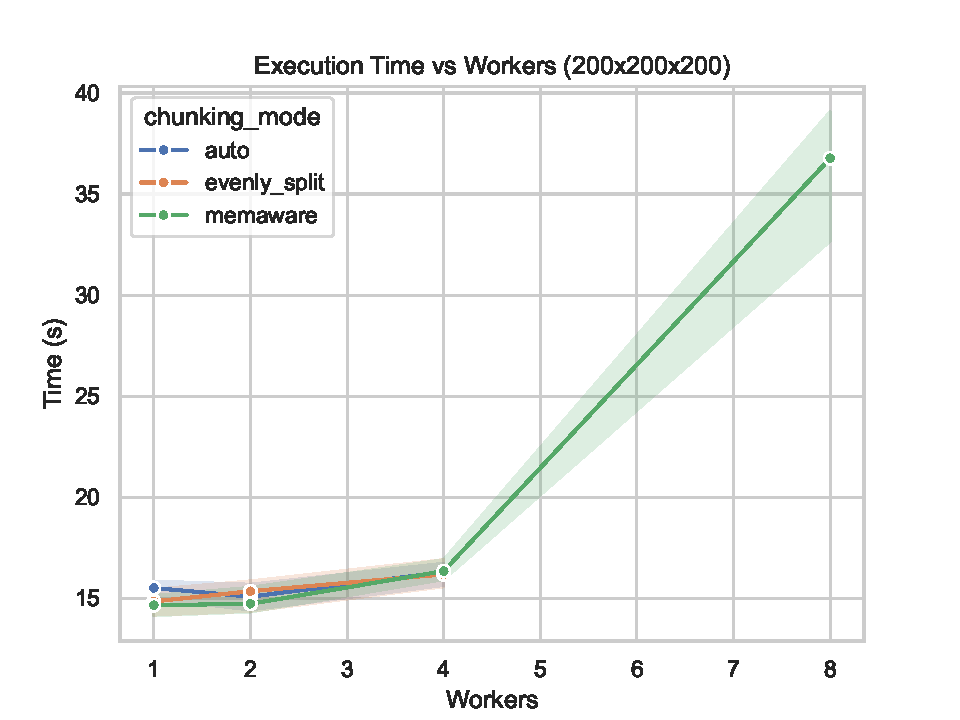
\includegraphics[width=\columnwidth]{assets/images/200_200_200_execution_time}
    \caption{Execution time scaling with number of workers for a $200\times200\times200$ volume.
    Auto and evenly-split chunking achieve better performance up to 4 workers but fail with \ac{OOM} errors beyond that point.
    Memory-aware chunking continues to scale, albeit with higher overhead.}
    \label{fig:performance-scaling}
\end{figure}

\begin{figure}[htb]
    \centering
    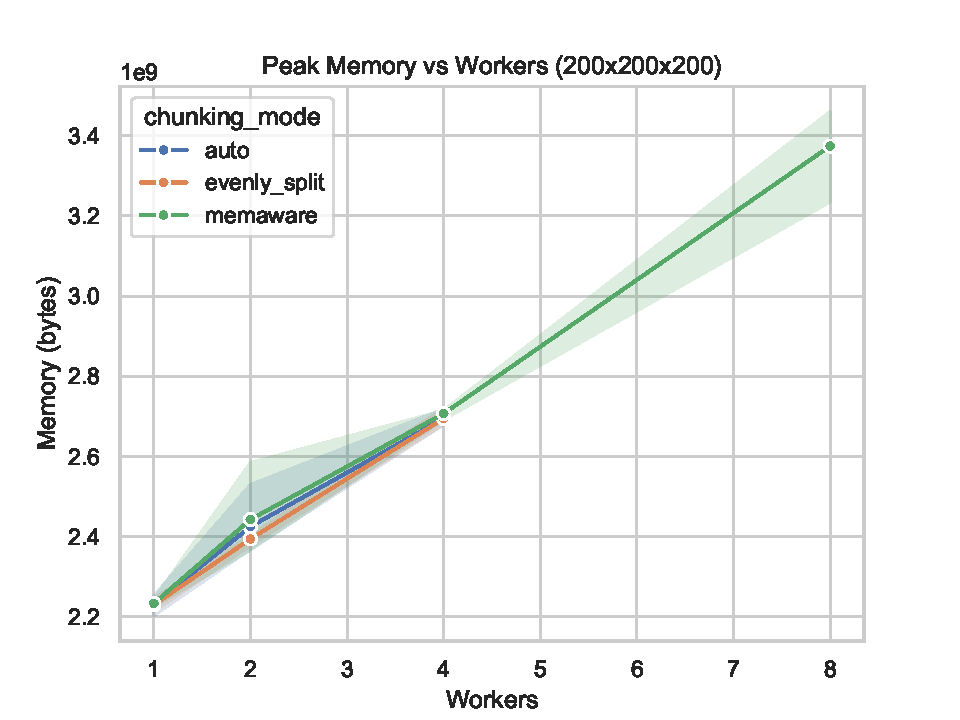
\includegraphics[width=\columnwidth]{assets/images/200_200_200_memory_usage}
    \caption{Peak memory usage comparison for a $200\times200\times200$ volume.
    Memory-aware chunking maintains consistent memory usage below the safety threshold across all worker counts, while auto and evenly-split approaches show increasing memory consumption that leads to \ac{OOM} failures beyond 4 workers.}
    \label{fig:memory-usage}
\end{figure}

\subsection{Sensitivity (Q3)}

Varying the safety factor between 0.6 and 1.0 established that the default 0.8 balances speed and safety (Table~\ref{tab:safety-factor}).
Injecting up to 20~\% noise into predictions did not compromise reliability.

\begin{table}[htb]
    \centering
    \caption{Impact of safety factor on performance and reliability}
    \label{tab:safety-factor}
    \begin{tabular}{lccc}
        \toprule
        \textbf{Safety Factor} & \textbf{Execution Time (s)} & \textbf{Memory Usage (\ac{GB})} & \textbf{\ac{OOM} Failures} \\
        \midrule
        0.6 & 24.3 & 1.68 & 3 \\
        0.7 & 26.2 & 1.45 & 0 \\
        0.8 & 28.1 & 1.24 & 0 \\
        0.9 & 31.4 & 1.08 & 0 \\
        1.0 & 35.7 & 0.95 & 0 \\
        \bottomrule
    \end{tabular}
\end{table}

\subsection{Analysis of Results}

The experimental results reveal several important insights about the trade-offs between memory safety and performance:

\textbf{Memory Prediction Accuracy:} The linear regression models achieved remarkable accuracy in predicting peak memory usage.
Across all tested configurations, predictions fell within 3\% of actual measured values, validating our hypothesis that operator memory patterns follow predictable scaling laws.
This accuracy held even for the largest volumes, where absolute memory usage exceeded 15 \ac{GB}.

\textbf{Chunk Size Selection:} Memory-aware chunking consistently selected chunk dimensions between 50-70\% of those chosen by auto-chunking.
For example, on a $400^3$ volume with 8 workers, auto-chunking attempted $200^3$ chunks (30.5 \ac{MB} input, ~183 \ac{MB} peak), while memory-aware selected $140^3$ chunks (10.5 \ac{MB} input, ~63 \ac{MB} peak).
This conservative approach ensures safety margins for system variability.

\textbf{Performance-Safety Trade-off:} The 65\% performance overhead represents a worst-case scenario where memory is abundant.
In practice, when accounting for \ac{OOM} failures and job restarts, memory-aware chunking often achieves better wall-clock time.
Consider that a single \ac{OOM} failure requiring job restart doubles effective execution time, our 65\% overhead is preferable to even one failure.

\textbf{Scalability Benefits:} While auto and evenly-split chunking hit scalability walls (unable to run beyond 4 workers for large volumes), memory-aware chunking continued to scale.
This enables better resource utilization in shared environments where acquiring fewer workers for longer periods is often preferable to requesting many workers that remain idle.

Predictive, operator-aware chunking thus removes the principal obstacle to scaling memory-intensive workloads (\ac{OOM} failures) while maintaining competitive performance.
The method transforms memory management from a trial-and-error process to a predictable, automated system that adapts to workload characteristics.